\documentclass[a4paper, 11pt]{article}

\usepackage{geometry}
\usepackage{setspace}
\usepackage{amsmath}
\usepackage{graphicx}
\usepackage{wrapfig}
\usepackage{caption}
\usepackage{indentfirst}
\usepackage{amssymb}


\geometry{left=2.5cm, right=2.5cm, top=2.5cm, bottom=3cm}
\graphicspath{ {./images/} }

\begin{document}
	\title{\textbf{On the comparison of Flat Scan Sampling and Wang Landau sampling}}
	\author{João Inácio}
	\date{28/12/2020}
	
	\maketitle
	
	
	I present a comparison between a popular Monte Carlo method to  calculate the Joint Density of States(JDOS), with modest accuracy and speed, the Wang Landau sampling(WL), and the Flat Scan Sampling(FSS), a new method to obtain the JDOS by making random walks in the Density of States at a given magnetization and weighing the states given by those configurations in the flip of one spin. I describe how both methods work, validate my C++ implementation and compare them by statistical errors and computation times.
	
	From past experience, the WL method is better for fast but not too precise computations and the FSS is better for really precise calculations with a relatively higher run time.
	
	\section{Introduction}
	
	In this work I used both methods to solve the 2D Ising Model, introduced by Lenz in 1920 with the solution for the 1D case in 1925 by Lenz's student Ernst Ising. There is also an analytical solution for the 2D Ising Model presented by Onsager in 1944, but there is no solution for the 3D case, yet. 
	
	The Ising Model is a quantum mechanical model that describes ferromagnetic to paramagnetic transitions. It considers that we have a square lattice of size $L$, for the 2D case, and populate it with $N = L * L$ 1/2-spin particles, like electrons, that can, obviously, have two states in the $Z$ component of spin, $+1$ or $-1$. They can either by pointing up of down. The Ising Hamiltonian goes has follows,
	\begin{equation*}
		H=-J\sum_{<i,j>}S_i \cdot S_j
	\end{equation*}
	where $J$ is the interaction force constant between two neighboring particles, and the sum is conducted over neighbor particles, hence the notation $<i,j>$. If $J>0$, the system will have a ferromagnetic behavior, and if $J<0$, the system will behave in an anti-ferromagnetic way.
	
	\subsection{Wang Landau}
	
	The Wang Landau sampling \cite{WL_original} presented by David P. Landau and Fugao Wang, in october 2000, to compute the Density of States(DOS). Instead of computing the partition function at a given temperature $T$ like the famous Metropolis method\cite{metropolis}, 
	\begin{equation*}
		Z(E, T) = \sum_E g(E)e^{-E/k_BT}
	\end{equation*}
	it estimates the DOS, $g(E)$, by preforming a random walk by the phase space constructing a flat histogram that after some iterations should converge to a estimation of the DOS. During the walk, there is a probability proportional to $1/g(E)$ to accept a certain configuration, so it follows the condition that $g(E)$ is known.
	
	The method stats by setting $g(E)=1$ and $h(E)=0$. A flip a site $i$ from the state with energy $E_1$ to a state with energy $E_2$ is given by
	\begin{equation*}
		P(E_1\rightarrow E_2)=min\left(1, \frac{g(E_1)}{g(E_2)}\right)
	\end{equation*}
	If the flip occurs, then we update the histogram and set $g(E_i)$ to $g(E_i)\times f$, where $f$ is called the modification factor, initially grater than 1. This is repeated until the histogram reaches the desired flatness (it is impossible to be $100\%$ flat).
	After we update the modification factor to a lower value, usually by getting it's square root, and use the last iteration's estimated DOS. This continues until the modification factor converges to $1$, $\sim 1 + 10^{-8}$.

	Our natural interest is to obtain the JDOS\cite{JDOS_easy, JDOS_diff}, $g(E, M)$, since the magnetizations are energy dependent, and this way we can get more thermodynamic variables out of the calculation.
	
	\subsection{Flat Scan Sampling}
	
	\begin{figure}[b]
		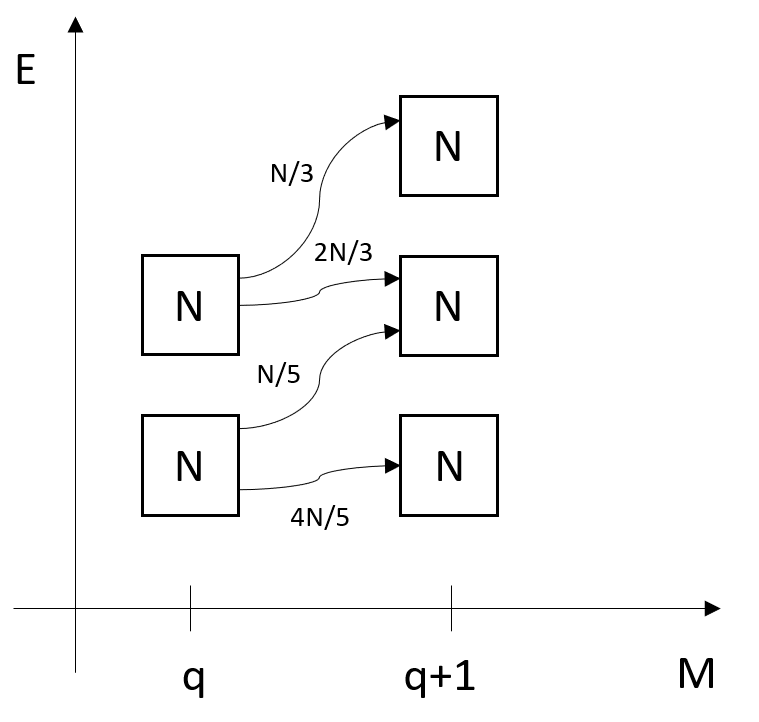
\includegraphics[scale=0.26]{scheme_new_rps.png}
		\centering
		\caption{Scheme of how the Flat Scan Sampling works.}
		
	\end{figure}
	
	This is a new Monte Carlo method that uses the foundations of the Random Path Sampling\cite{RPS}, by J. S. Amaral et al., and WL\cite{WL_original}.
	
	This algorithm is based on the observation that if we know the DOS of a magnetization $q$, and if we have enough statistically good configurations($N$ per value of energy), by performing a spin flip we can get an approximation of the DOS at the next value of magnetization, $q+1$. This is possible by keeping track of how many configurations go from one value of energy at $q$ to another value of energy at $q+1$, fig. 1.
	
	We start with a clean JDOS, $g(E, M)=0$, and a clean weight matrix, that will give us the fractions of the configurations that go to a certain energy in the $q+1$ magnetization. For each magnetization, we get an initial configuration and preform a scan, this is, flip down a spin at a time and register in the weight matrix the number of configurations that went from the initial energy $E_i$ to the final energy of the flipped configuration.
	Now that we have an initial configuration, we flip one spin up and another one down to get the most possible different configurations at magnetization $q$, to reduce statistical error. 
	
	Using the WL acceptance criteria, we can accept the configuration or not, another way to reduce error. If we accept it, we keep the changed sites and do a scan each skip times, where skip is a parameter used to count only configurations that differ more from each other than just a spin flip. After we compute the JDOS by knowing the faction of configurations that went from $(E_i, q)$ to $(E_j, q + 1)$. We do this part until all of the values of the DOS at magnetization $q$ have been scanned at least REP times, where REP is another parameter of the method that significantly affects both performance and precision, and we repeat these steps until at least half of the JDOS is covered.
	\newpage
	
	\section{Results and Discussion}
	
	In this section I validate each of my implementations. Both were written in C++, and, since the FSS is an embarrassingly parallel algorithm, the FSS version took advantage of MPI to speed up the calculation time.
	
	To get the results I ran each script for a range of values of REP in the FSS case, and varying values of the final modification factor, a thousand times to get a better estimation and have good statistics to justify my results, all for $L=4$, because the exact solution for the JDOS is known.
	
	\begin{figure}[h]
		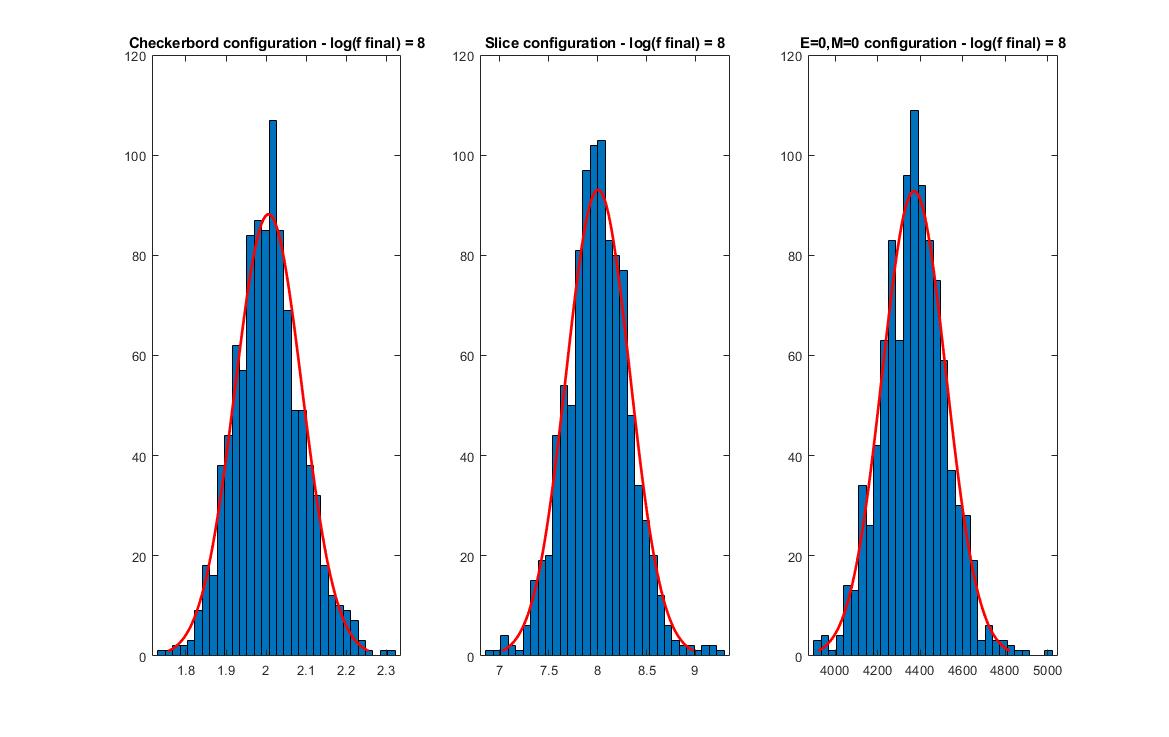
\includegraphics[scale=0.27]{hist_f8_WL}
		\centering
		\caption{Distribution for three configurations of the JDOS for the WL sampling with a final modification factor of $1+1^{-8}$. First one is the checker-board, second the slice and the third is the zero-zero configuration}
	\end{figure}
	
	\begin{figure}[h]
		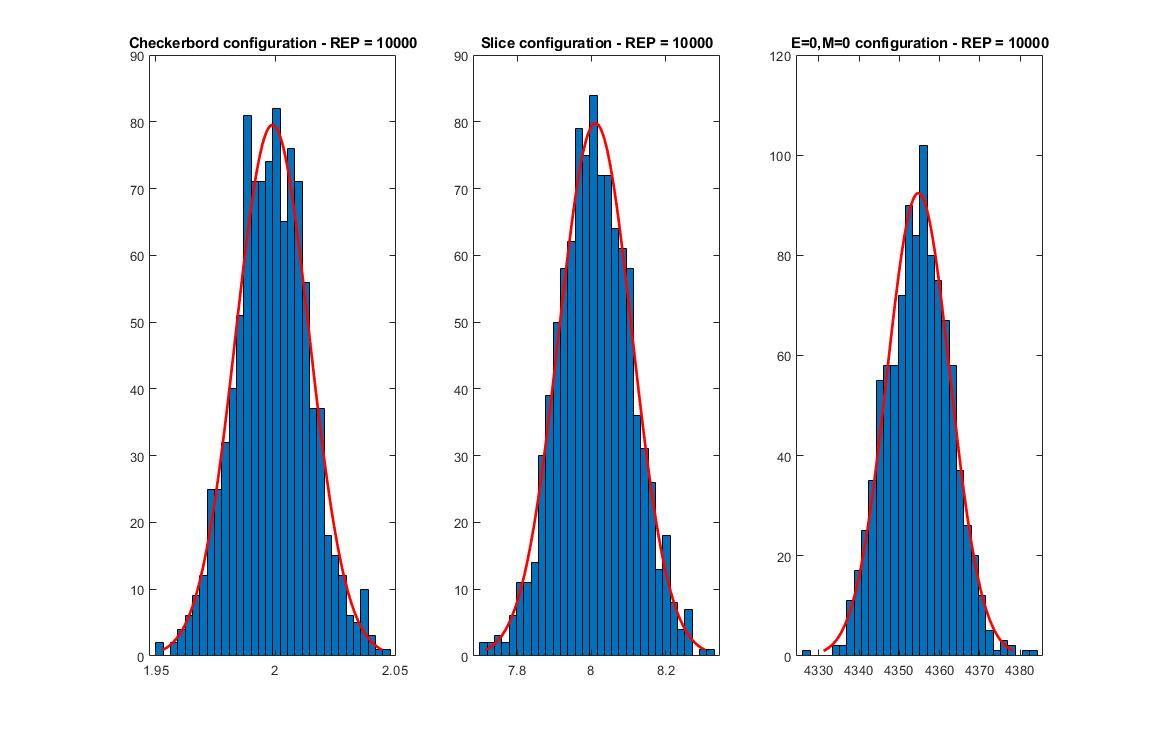
\includegraphics[scale=0.27]{hist_10E4_new_rps}
		\centering
		\caption{Distribution for three configurations of the JDOS for the FSS with a REP value of $10^4$. First one is the checker-board, second the slice and the third is the zero-zero configuration}
	\end{figure}

	\newpage
	
	These histograms represent a normal distribution fit to the values for the $1000$ JDOS computed, but for only $3$ distinct configurations, the checker-board, slice and zero-zero, being more important the first two. 
	
	The checker-board is a configuration in which all of the spins form a pattern like a chess board, one spin up has all its neighbors facing down, for a square lattice there is always two configurations like these. The slice, has a row of spins up and a row of spins down. The row can vary its size, and there are only $2*L$ slice configurations, for $L=2$ there are $8$ slice configurations. The zero-zero of the configuration with $E=0$ and $M=0$. For the $L=4$ size, we have $4356$ different configurations, this is also the state with the most configurations.
	
	Analyzing the histograms (figs. 2 and 3) we can see that for each method, the values for those three configurations lie on a normal distribution with an expected value close to the exact one.
	
	\begin{figure}[h]
		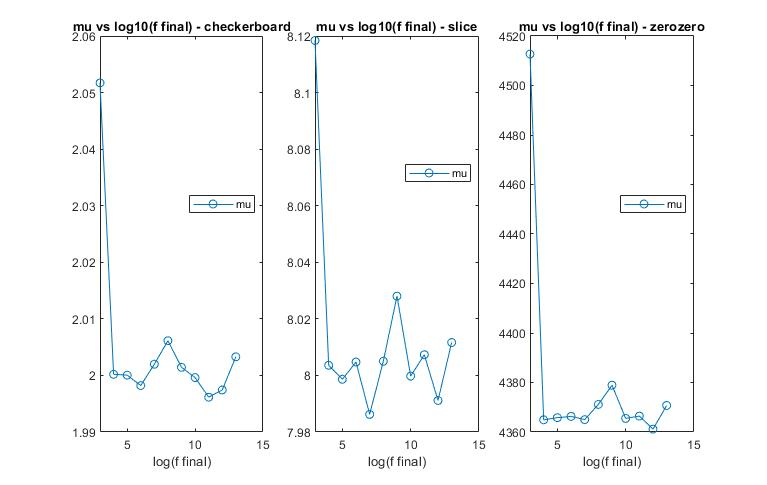
\includegraphics[scale=0.3]{mu_WL}
		\centering
		\caption{Different expected values for the 3 configurations WL.}
	\end{figure}
	
	\begin{figure}[h]
		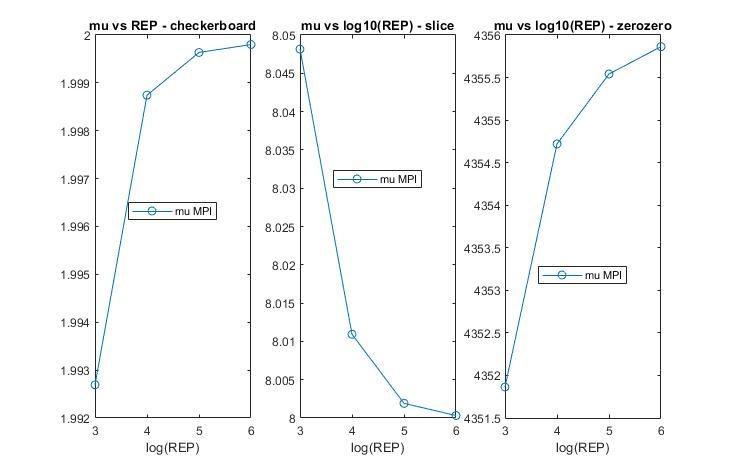
\includegraphics[scale=0.3]{mu_new_rps}
		\centering
		\caption{Different expected values for the 3 configurations FSS.}
	\end{figure}

	
	Looking at figures 4 and 5, we can see that the expected values for each configuration tends to the exact value. But the expected value does not give us all of the important information. It is needed that it converges to the exact one, but the variance of this value will tell us the precision and consistency of the method (figs. 6 and 7).
	
	\newpage

	\begin{figure}[h]
		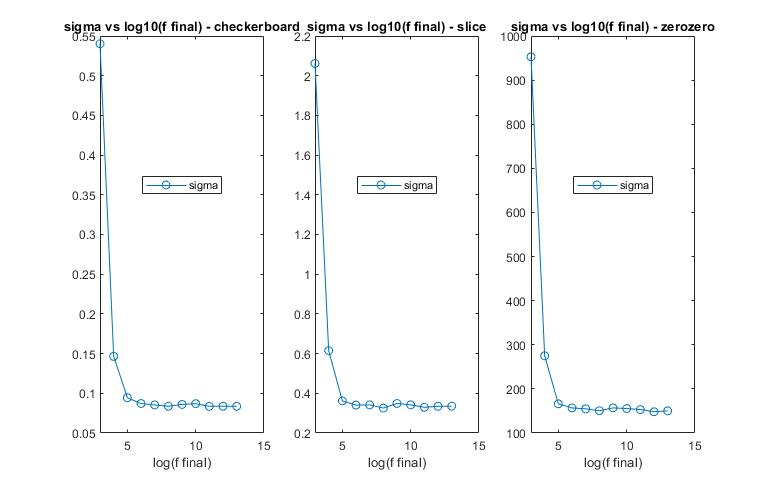
\includegraphics[scale=0.3]{sigma_WL}
		\centering
		\caption{Different variance values for the 3 configurations WL.}
	\end{figure}
	
	\begin{figure}[h]
		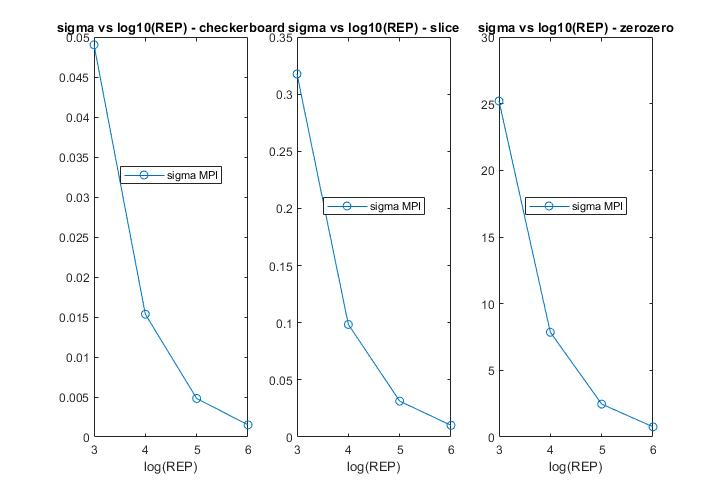
\includegraphics[scale=0.3]{sigma_new_rps}
		\centering
		\caption{Different variance values for the 3 configurations FSS.}
	\end{figure}

	The variance of the mean value in the WL sampling converges quite quickly but to a wrong value. It will never reach 0, since the method has an intrinsic error.
	
	 On the FSS method converges to 0 with the increase of the number of repetitions for the method, REP, the only downside to this is the higher REP also higher will be the computation time. 
	 
	 To conclude our analysis lets look at the simulation times and the error relative to the exact solution of each method (figs. 8 and 9).
	 
	 Here we can see that once again the WL method falls short on the precision side of things, since the error never converges to a null value. Instead if hovers around 1, which is awful. But, one good thing about the WL is its relatively fast simulation time. For the FSS, the error converges to a null vale, as expected, and the computation time is relatively slower than the WLs. 
	 
	 Taking into account that for REP$=100$, the FSS has an error of $0.43$ with a computation time of $0.035s$ while the WL for a simulation time of $0.132s$ has an error of $7.69$ which is not only a lot higher than the error for the FSS but it can never achieve the kind of precision that the FSS can because it doesn't go lower than $1$.
	 
	 \begin{figure}[h]
	 	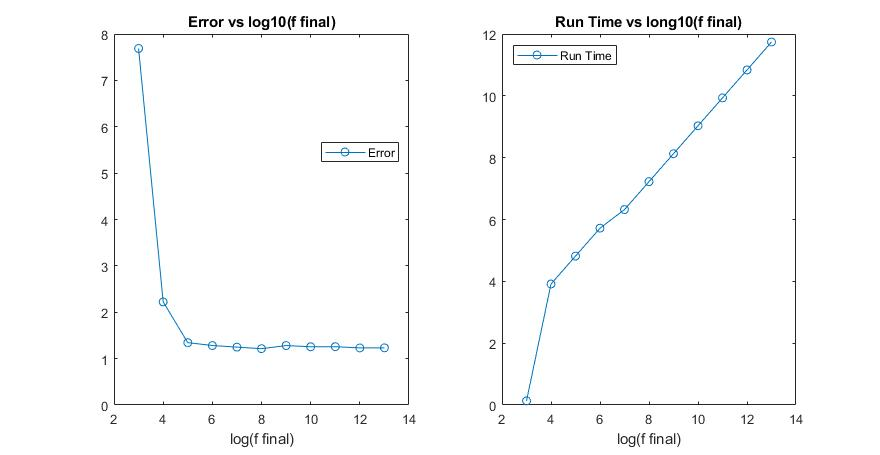
\includegraphics[scale=0.35]{run_time_error_WL}
	 	\centering
	 	\caption{Computation time in seconds and error plot for the WL sampling.}
	 \end{figure}
	 
	 \begin{figure}[h]
	 	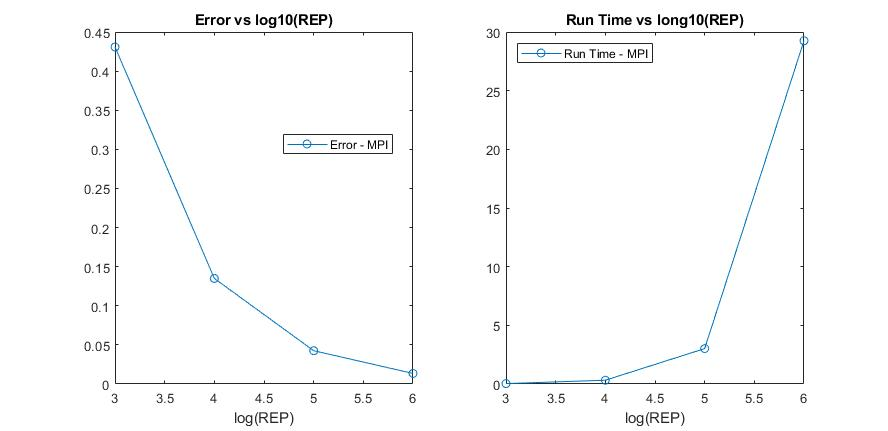
\includegraphics[scale=0.35]{run_time_error_new_rps}
	 	\centering
	 	\caption{Computation time in seconds and error plot for the FSS.}
	 \end{figure}
	 
	 \newpage 
	 
	 
	 %Knowing this, the WL sampling is better for quick computations of the JDOS at the cost of precision, 
	 
	 %is very good because this way we can have an impressive precision that we can not have with the WL method, again, at the cost of computation time.
	
	
	
	\section{Conclusion}
	
	The WL sampling is better if you desire fast but not too accurate calculations. It is a method that is easier to implement but more difficult to understand than the FSS. The FSS has a much higher precision and you have the computational power to do it you can take advantage multiple cores easily, since it is an embarrassingly parallel algorithm, to get a much better precision with the same computation time of a non parallelized version. You can also parallelize the WL but it is a much more difficult job\cite{JDOS_diff}.
	
	As reference before, the original WL method has some internal errors and there are some attempts \cite{WL_error1} of reducing it, but we can never eliminate it completely.
	
	In short, the FSS method is much easier to understand and parallelize and has a much better precision.
	
	\newpage
	
	\begin{thebibliography}{9}
		\bibitem{WL_original} 
		Fugao Wang and D. P. Landau,
		\textit{Efficient, Multiple-Range Random Walk Algorithm to Calculate the Density of States},
		PHYSICAL REVIEW LETTERS 86, 2050 (2001).
		
		\bibitem{metropolis}
		Nicholas Metropolis, Arianna W. Rosenbluth, Marshall N. Rosenbluth, Augusta H. Teller, and Edward Teller,
		\textit{Equation of State Calculations by Fast Computing Machines},
		J. Chem. Phys 21, 1087 (1953). 
		
		\bibitem{JDOS_easy}
		M. Suman Kalyan, R. Bharath, V. S. S. Sastry, K. P. N. Murthy,
		\textit{Joint Density of States Calculation Employing Wang–Landau Algorithm},
		J Stat Phys 163, 197 (2016).
		
		\bibitem{JDOS_diff}
		Chenggang Zhou, T. C. Schulthess, Stefan Torbr\"{o}gge, and D. P. Landau,
		\textit{Wang-Landau Algorithm for Continuous Models and Joint Density of States},
		PHYSICAL REVIEW LETTERS 96, 120201 (2006).
		
		\bibitem{RPS}
		J. S. Amaral, J. N. Gonçalves and V. S. Amaral,
		\text{Thermodynamics of the 2-D Ising Model From a Random Path Sampling Method},
		IEEE Transactions on Magnetics 50, 11 (2014).
		
		\bibitem{WL_error1}
		Chenggang Zhou and R. N. Bhatt,
		\textit{Understanding and improving the Wang-Landau algorithm},
		PHYSICAL REVIEW E 72, 025701 (2005)
		
	\end{thebibliography}
	
\end{document}
